% 0151(본책 33쪽) — 직각삼각형 ABC(∠A=90°, ∠B=45°), AB=x·AC=4·BC=y. 스캔 삽화를 TikZ 로 다시 그림. 빈칸 답은 적지 않는다.
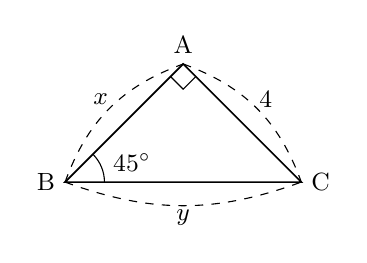
\begin{tikzpicture}[line width=0.6pt]
  \coordinate (B) at (0,0); \coordinate (C) at (3,0); \coordinate (A) at (1.5,1.5);
  \draw (A) -- (B) -- (C) -- cycle;
  \draw[line width=0.4pt] (1.34,1.34) -- (1.5,1.18) -- (1.66,1.34);
  \draw[line width=0.4pt] (0.5,0) arc[start angle=0, end angle=45, radius=0.5];
  \node[font=\small] at (0.85,0.25) {$45^\circ$};
  \draw[dashed, line width=0.4pt] (B) to[bend left=25] (A);
  \draw[dashed, line width=0.4pt] (A) to[bend left=25] (C);
  \draw[dashed, line width=0.4pt] (B) to[bend right=20] (C);
  \node[font=\small] at (0.45,1.05) {$x$};
  \node[font=\small] at (2.55,1.05) {$4$};
  \node[font=\small] at (1.5,-0.45) {$y$};
  \node[font=\small, above] at (A) {A};
  \node[font=\small, left] at (B) {B};
  \node[font=\small, right] at (C) {C};
\end{tikzpicture}
